\documentclass[]{report}
\usepackage{pdfpages}
%\usepackage{amsmath}
\begin{document}
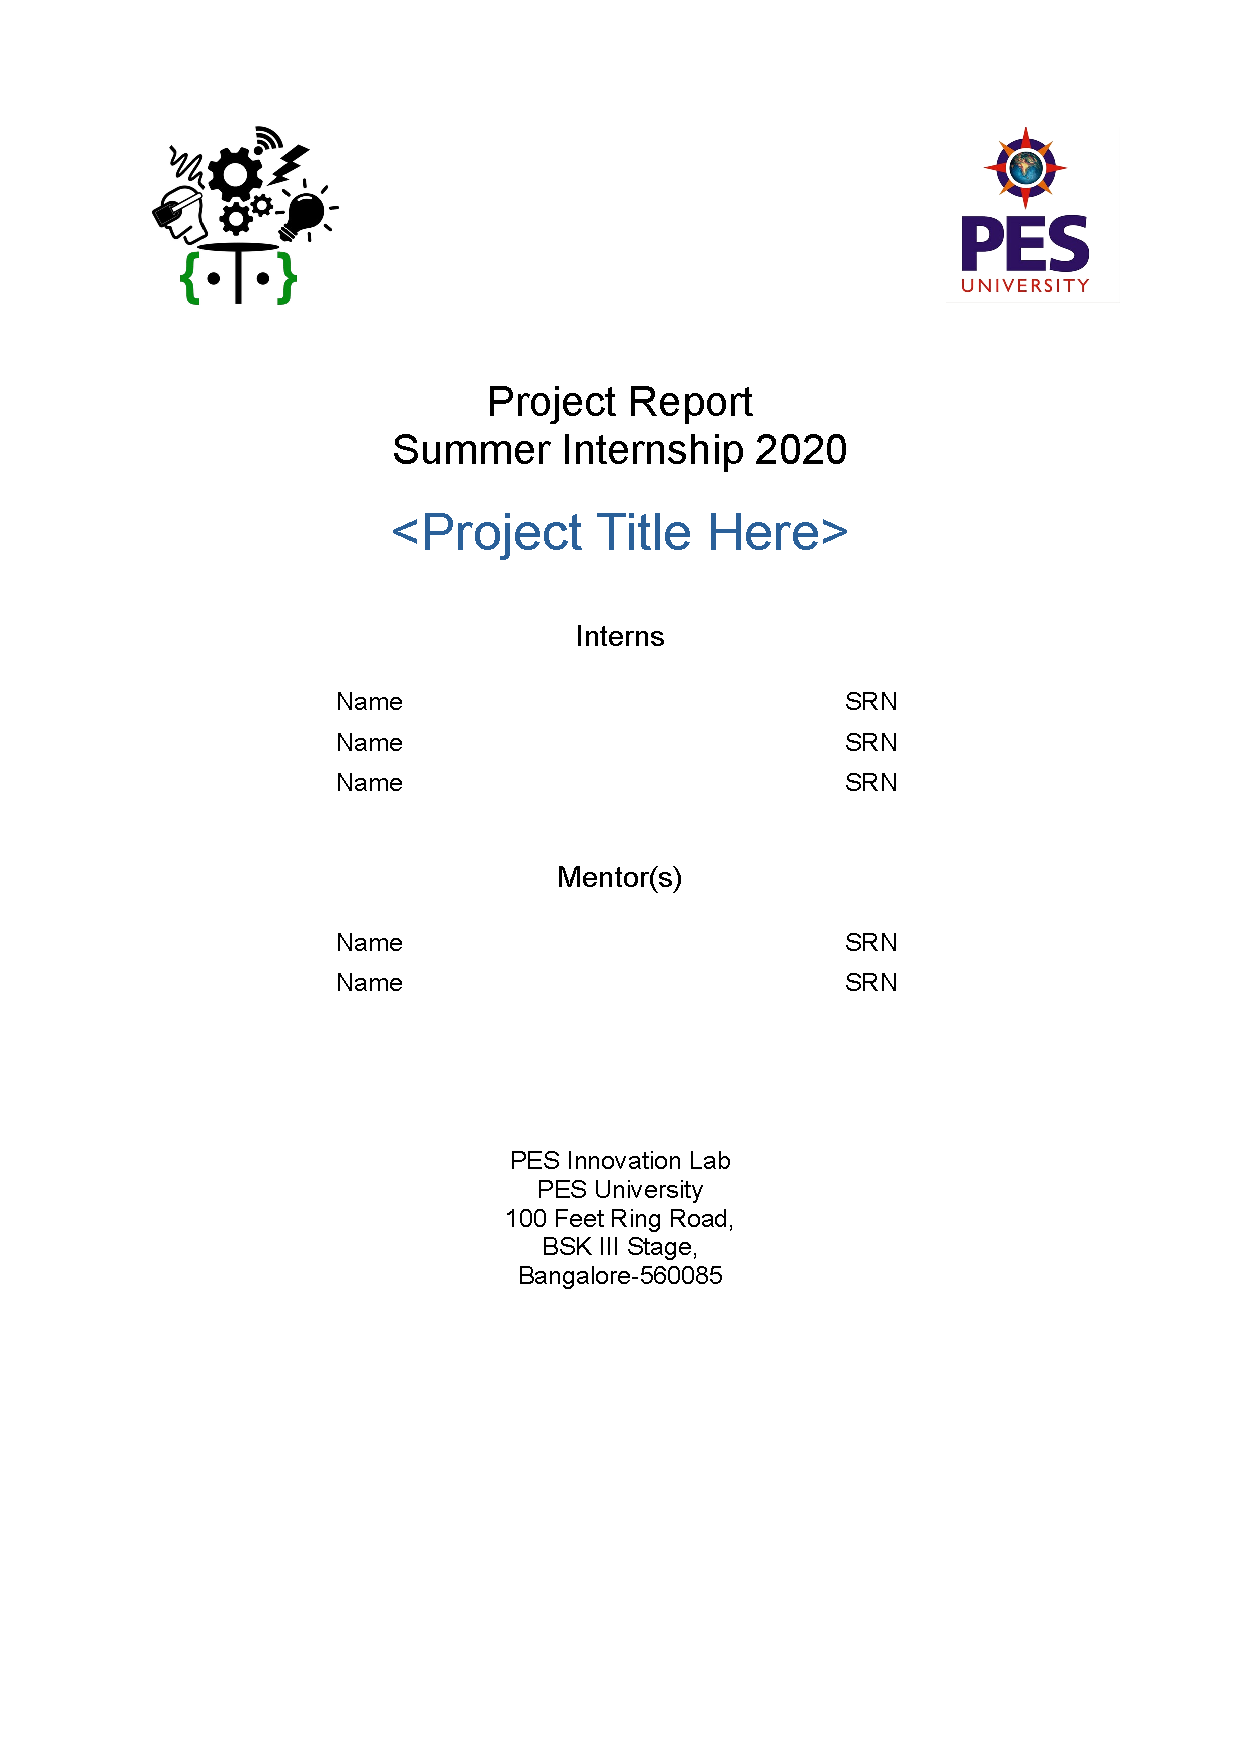
\includepdf[pages={1}]{coverpage.pdf} 

\begin{abstract}
 
\end{abstract}

\tableofcontents
%\listoffigures
%\listoftables

\chapter{Introduction}
Length: [0.5 to 2 pages ]
Introduce the reader to the problem/domain. Write about the issues that your project addresses/improves/solves. Write about use-cases for your project. 
\section{Problem Statement}
A formal statement of what you are trying to achieve. \\

You can conclude the introduction by writing how the rest of the report is organised.

\chapter{Literature Survey/Related Work} 
Length: [1-3 pages]. 
Are there existing solutions to your problem? If yes, elaborate in a few lines. You can also write about the theory/concepts associated with your project. Cite related work  \cite{wiki:latex}.  You can conclude this section by stating how your work is novel/different from the related work you have just described. For each paper or link that you mention here, please include a short summary of the resource as well as how the resource contributed to your project.

\chapter{Main Body}d
This is the heart of your report. It describes your project. It can be more than one chapter/section. For example : 'System model', 'methodology', 'solution method', 'approach'. Include diagrams, flow charts, algorithms etc. if relevant. Make sure you refer to all figures and tables that you include in the text. Like this: In Figure \ref{solvay}, the IQ level is over 9000! (Read in Vegeta voice.)
%template for figure

\begin{figure}[ht]
  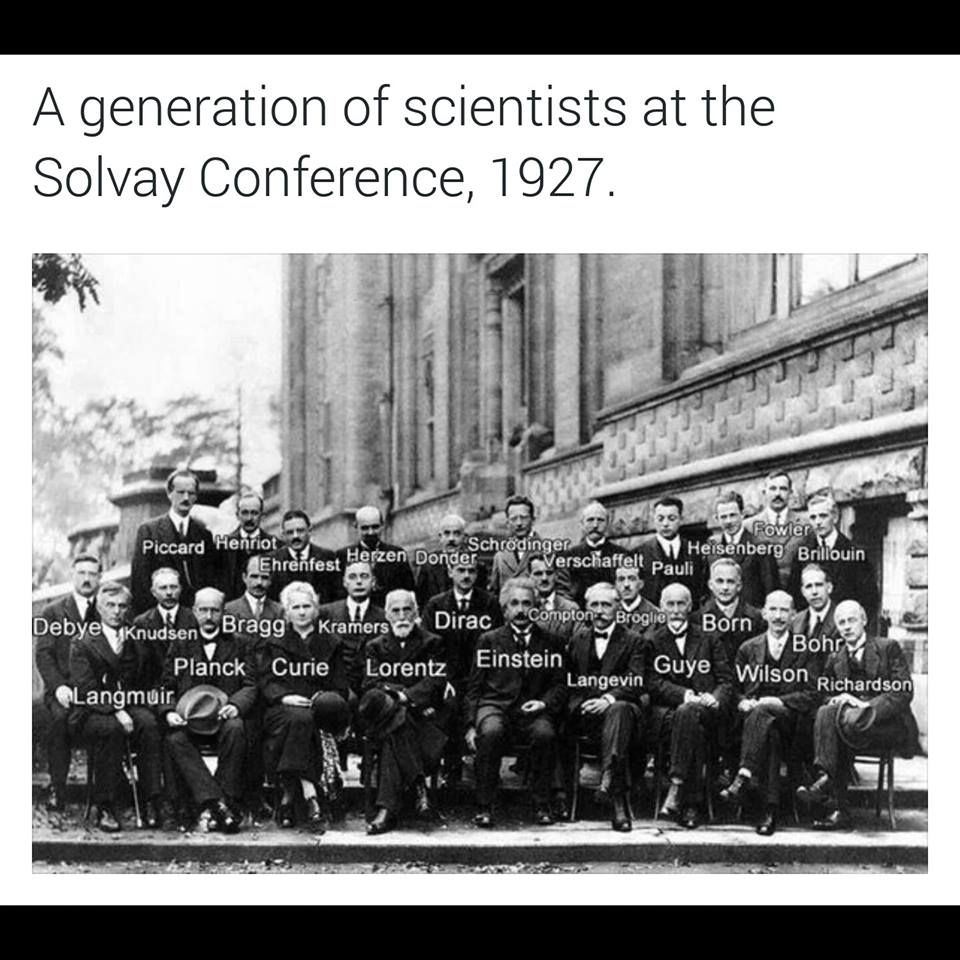
\includegraphics[width =\columnwidth]{solvay.jpg}
  \caption{Some inspiration}
  \label{solvay}
\end{figure}

\section{Hardware and Software Requirements}
What hardware/software did you use? Can be lists or tables if you used many. Mention version numbers of software. Mention stats. of the computer you did your project on. 

\chapter{Results and Discussion}
Include tables (see Table \ref{XYComparison} for a template), figures and plots to represent your results if possible. What were the key outcomes? Do they match with expected results? Why/why not? Discuss and explain results where possible. Talk about challenges faced and the limitations of the present implementation if any. 
%template for table
\begin{table}[ht]
\label{XYComparison}
\begin{center}
\begin{tabular} {l|l|l} %left aligned
\hline
\hline
\textbf{Criteria} & \textbf{X} & \textbf{Y}  \\
\hline
A & B & C \\
D & B & C \\
\hline 
\hline
\end{tabular}
\end{center}
\caption{Comparison of  X and Y}
\end{table}

\chapter{Conclusions and Future Work}
A short paragraph about the conclusions you have drawn. Feel free to change the formatting and sizes of your figures/tables. In conclusion, your report should a) give the reader an idea of what you did b) allow them to understand and replicate your results.

%Please make sure you keep a log of all the resources you have used. This includes websites, tutorials, videos, papers or even blogs can be cited.

\bibliographystyle{ieeetr} 
\bibliography{bibmil.bib}
\appendix 
\chapter{sample appendix header 1}
%\label{app_1}
Appendices: 
Proofs, links to your code and any other misc. info that doesn?t fit in nicely into other sections. 


\end{document}
